\newpage
\section{Auswertung}
\subsection{Der Acrylquader}
Die aufgenommenen Daten des Acrylquaders befinden sich in Tabelle \ref{tab:1}.
\begin{table}
    \centering
    \caption{Messwerte des Acrylquaders.}
    \begin{tabular}{c c c c}
        \toprule
        {Nr.} & {$d \, / \, \si{\milli\meter}$} & {$t \, / \, \si{\micro\second} $} & {$I \, / \, \si{\volt}$} \\
        \midrule
     1  & 59.60    &    44.4   &     0.22\\
     2  & 61.21   &    44.7   &     0.23\\
     3  & 13.49   &    10.5   &     1.27\\
     4  & 21.60    &    16.7   &     1.13\\
     5  & 30.10    &    22.7   &     0.85\\
     6  & 38.80    &    29.3   &     0.54\\
     7  & 46.80    &    35.2   &     0.43\\
     8  & 54.70    &    40.8   &     0.25\\
     9  & 62.70    &    46.7   &     0.24\\    
     10 & 70.90    &           &         \\
     11 & 15.80    &    12.0     &     1.23\\
        \bottomrule
    \end{tabular}
    \label{tab:1}
\end{table}

\noindent
Dabei ist anzumerken, dass Störung Nr. 10 mit dem Impuls-Echo-Verfahren (IEV) nicht zu erreichen ist, 
da die Schallwellen bereits an Störung Nr. 11 reflektiert werden. \\

\noindent
\textbf{Vermessung mit dem IEV}

\noindent
Die mit der Schiebelehre gemessenen Abstände werden nun mit dem IEV überprüft.
Dabei wird eine Schallgeschwindigkeit in Acryl von $c_{lit} = 2730 \si[per-mode=fraction]{\meter\per\second}$ angenommen.
Die Abstände werden nach Formel () bestimmt und sind in Tabelle \ref{tab:2} aufgeführt. %formel s=0.5ct wk,suzjgvdhcadiufzjsdiefuwghjddfghjufzgjhuefgzjuhzgvm

\begin{table}
    \centering
    \caption{Gemessene Tiefen der Störungen mit dem IEV.}
    \begin{tabular}{c c}
        \toprule
        {Nr.} & {$d_{IEV} \, / \, \si{\milli\meter}$} \\
        \midrule
     1  & 60.61  \\
     2  & 61.02 \\
     3  & 14.33 \\
     4  & 22.80  \\
     5  & 30.99  \\
     6  & 40.00 \\
     7  & 48.05  \\
     8  & 55.70  \\
     9  & 63.75  \\    
     10 &       \\
     11 & 16.34 \\
        \bottomrule
    \end{tabular}
    \label{tab:2}
\end{table}

\noindent
\textbf{Schallgeschwindigkeit}

\noindent
Die Schallgeschwindigkeit in Acryl kann mit Formel ()%formel s=0.5ct kjehfeauhfaghfjsegrykdjhdruwzefgchbsjduhdfjksawefhuzfgsbchjawidufzgjvhelikjggh
bestimmt werden.
Dazu werden die Messwerte aus Tabelle \ref{tab:1} verwendet.
Wird der doppelte Abstand $d$, die Strecke die der Ultraschall tatsächlich zurücklegt,
gegen die Zeit $t$ geplottet die er dafür benögtigt, ist die Steigung der Ausgleichsgeraden
die Schallgeschwindigkeit.


\noindent
Mittels Python kann die Ausgleichsgerade mit der aus numpy \cite{numpy} importierten Funktion polyfit bestimmt werden.
Diese ist in Abbildung \ref{fig:schall} dargestellt.

\begin{figure}
    \centering
    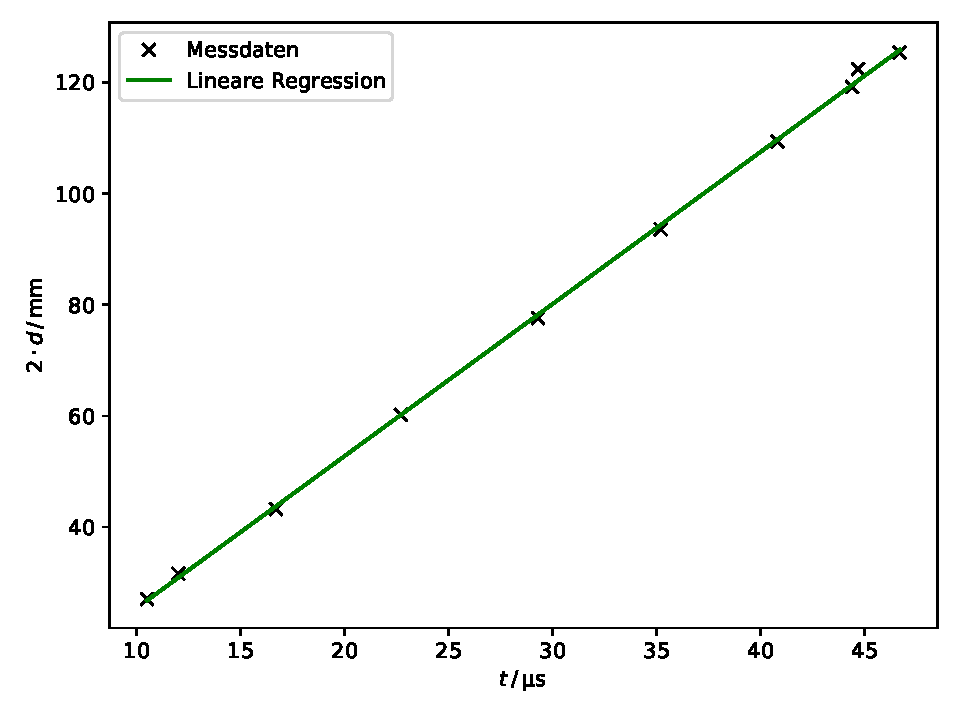
\includegraphics[width=11cm]{Daten/schall.pdf}
    \caption{Ausgleichsgerade zur Bestimmung der Schallgeschwindigkeit (Quelle:\cite{US1}).}
    \label{fig:schall}
  \end{figure}
  
\noindent
Die Ausgleichsgerade hat dabei die Funktionsvorschrift:

\begin{align*}
2 \cdot d(t) &= 2.7372 \, \si[per-mode=fraction]{\milli\meter\per\micro\second} \cdot t \\
\implies c_{Acryl} &= 2732.2 \, \si[per-mode=fraction]{\meter\per\second} \\
\end{align*}

\noindent
\textbf{Dämpfungskonstante}

\noindent
Die Dämpfungskonstante $\alpha$ aus Formel () lässt sich bestimmen, indem die Messwerte für $I$ und $d$ aus Tabelle \ref{tab:1} an eine Exponentialfunktion gefittet werden. %Formel I(t)= e^-ax bla bla liehvfkesjrhgkaervskejbkjb
Mit Python kann eine e-Funktion mit passenden Parametern mit der aus scipy \cite{scipy} importierten Funktion curvefit bestimmt werden.

\begin{figure}
    \centering
    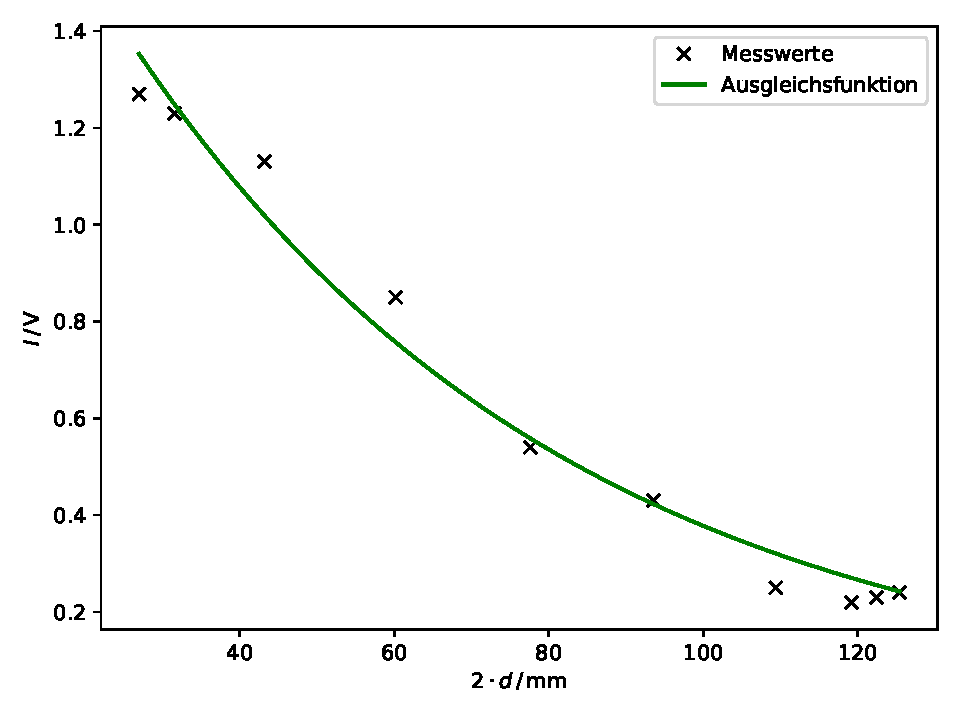
\includegraphics[width=11cm]{Daten/daempf.pdf}
    \caption{Ausgleichsfunktion zur Bestimmung der Dämpfungskonstante (Quelle:\cite{US1}).}
    \label{fig:daempf}
  \end{figure}

  \newpage
\noindent
Die in Abbildung \ref{fig:daempf} dargestellt Ausgleichsfunktion hat die Funktionsvorschrift:

\begin{align*}
I(d) &= 2.167 \, \si{\volt} \cdot e^{-0.0175 \, \si[per-mode=fraction]{\per\milli\meter} \cdot 2 \cdot d}\\
\implies \alpha &= 17.5 \, \si[per-mode=fraction]{\per\meter}\\
\end{align*}


\subsection{Das Augenmodell}
Bei der Untersuchung des Augenmodells wurden 3 Peaks aufgenommen.
Der erste und zweite Peak entstehen beim eintreffen und ausfallen der Linse, der dritte durch Reflexion an der Retina.
Unter Berücksichtigung der Schallgeschwindigkeit in der Linse ($c_L = 2500 \si[per-mode=fraction]{\meter\per\second}$) und in der Glaskörperflüssigkeit
($c_{GK} = 1410 \si[per-mode=fraction]{\meter\per\second}$) kann aus der Laufzeit mit () die Strecke berechnet werden. %formel s=0.5ct xxxxxxkurfhaeolrufhefhekarguhkeugeksghrkgthrkugtrghrttkhjhgk
In Tabelle \ref{tab:auge} befinden sich die Messwerte und die daraus resultierenden Maße des Auges.

\begin{table}
    \centering
    \caption{Messwerte und Maße des Augenmodells.}
    \begin{tabular}{c c c c}
        \toprule
        {} & {$t \, / \, \si{\micro\second}$}& {Schallgeschwindigkeit} & {$d \, / \, \si{\milli\meter} $} \\
        \midrule
     \text{Hornhaut-Linsenvorderseite}  & 11.6 & $c_{GK}$ & 8.178 \\
     \text{Linsenvorderseite-Rückseite}  & 5.7 & $c_L$ & 7.125 \\
     \text{Linsenrückseite-Retina}  & 8.2 & $c_{GK}$ & 5.781 \\
        \bottomrule
    \end{tabular}
    \label{tab:auge}
\end{table}